\documentclass[11pt,letterpaper]{article}
 
% ---------- Packages ----------
\usepackage[margin=1in]{geometry}
\usepackage[T1]{fontenc}
\usepackage{lmodern}
\usepackage{microtype}
\usepackage{amsmath,amssymb}
\usepackage{booktabs}
\usepackage{graphicx}
\usepackage{float}
\usepackage{caption}
\usepackage{enumitem}
\usepackage{xcolor}
\usepackage{titlesec}
\usepackage{fancyhdr}
\usepackage[hidelinks]{hyperref}
\usepackage{siunitx}
\newcommand{\hyponote}[1]{{\footnotesize\itshape #1\par}}
 
\definecolor{gatorblue}{HTML}{0021A5}
\definecolor{gatororange}{HTML}{FA4616}
 
\titleformat{\section}{\large\bfseries\color{gatorblue}}{\thesection}{0.6em}{}[\color{gatororange}\titlerule]
\titleformat{\subsection}{\normalsize\bfseries}{\thesubsection}{0.6em}{}
\setlist{itemsep=1pt, topsep=2pt}
\titlespacing*{\section}{0pt}{7pt}{4pt}
\titlespacing*{\subsection}{0pt}{5pt}{2pt}
\titlespacing*{\subsubsection}{0pt}{4pt}{2pt}
\titlespacing*{\paragraph}{0pt}{4pt}{6pt}
\captionsetup{skip=3pt}
\setlength{\textfloatsep}{8pt}\setlength{\floatsep}{6pt}\setlength{\intextsep}{6pt}
 
\pagestyle{fancy}
\fancyhf{}
\cfoot{\small\thepage}
\renewcommand{\headrulewidth}{0pt}
 
% ---------- Metadata ----------
\newcommand{\NoteTitle}{Algorithmic Genetic Feature Selection to Improve XGBoost on E-mini S\&P~500 Order-Book Data.}
\newcommand{\Authors}{Manny Osorio, Emily Diaz-Silva, Benjamin Friedman}
\newcommand{\NoteDate}{\today}
\newcommand{\TeamName}{Gator Quant Hacks Team}
 
\begin{document}
 
% ---------- Title block ----------
\begin{center}
    {\LARGE\bfseries\color{gatorblue} \NoteTitle}\\[6pt]
    {\large Quant Note -- Systematic Trading Track}\\[4pt]
    \Authors
\end{center}
 
% ============================================================
\section{Summary}
% ============================================================
\textbf{Overall Strategy:} On each ES order-book update, we combine GA-selected book features and XGBoost outputs into a standardized score. If it clears a cost-based threshold, we execute a one-contract market position and exit after a fixed holding window.
 
We evaluate whether the ten-level order book of the CME E-mini S\&P~500 future (ES) predicts mid-price direction over the next $h=1.5$ seconds better than a top-of-book rule. An XGBoost model estimates move probabilities from 25 book-state features, while a GPU-accelerated genetic algorithm (GA) searches for the feature subset, entry threshold, and lookback. The frozen rule is replayed out-of-sample in an event-driven simulator using recorded order books. Net of fees, the strategy achieves 2{,}547 trades with a mean net P\&L of \$2.50 per trade, a net Sharpe ratio of 1.58, and a maximum drawdown of 4.3\% over 63 days, comparing against random and level-1 baselines.\footnote{\textbf{All performance figures in this paper are hypothetical and illustrative; they were not produced by our pipeline.} The SHAP plots in Appendix~\ref{app:shap} are the only model outputs shown.}
 
% ============================================================
\section{Economic and Data Hypothesis}
% ============================================================
 
\subsection{Economic Hypothesis}
The ten-level ES order book contains microstructural information regarding mid-price direction over $h$ seconds. Because market makers update quotes with latency and manage adverse-selection risk, temporary volume imbalances briefly misplace prices. Aggressive traders and stale market makers absorb these costs. Edge persists because liquidity provision requires bearing adverse selection, limiting capital competition.
 
\paragraph{Testable prediction.} Net of spread and fees, the frozen rule earns positive out-of-sample returns; realized returns scale across buckets of the model's directional score; and the rule beats random feature subsets and level-1 imbalance rules.
 
\paragraph{It fails if.} (1) Out-of-sample net returns are negative after transaction costs; (2) realized returns are non-monotone relative to directional scores; or (3) performance fails to beat baselines.
 
% ============================================================
\section{Data and Universe}
% ============================================================
We trade a single instrument: the CME E-mini S\&P~500 front-month future (\texttt{ES.c.0}, ESH4 contract). Market data comes from Databento~\cite{Databento} (\texttt{GLBX.MDP3}, \texttt{mbp-10} schema) at nanosecond resolution. The sample spans 2024-01-08 to 2024-07-08, containing $1.14\times10^{9}$ book events. 

We utilize \texttt{ts\_recv} timestamps. Crossed/locked books are dropped, empty levels are padded with zeros, and maintenance breaks (17:00--18:00 ET) are excluded.
 
% ============================================================
\section{Methodology}
% ============================================================
\subsection{Model Training and Genetic Search}
\paragraph{XGBoost.} The gradient-boosted tree classifier~\cite{chen2016xgboost}
(GPU histogram method, \texttt{multi:softprob}, three classes) outputs
$[P_{\text{sell}},P_{\text{hold}},P_{\text{buy}}]$. Out-of-fold probabilities are produced with an expanding-window purged walk-forward scheme. The directional score is $q_i = P_{\text{buy}}(\mathbf{x}_i) - P_{\text{sell}}(\mathbf{x}_i) \in [-1,1]$.
 
\paragraph{Genome.} Encoded as a 64-bit chromosome (Table~\ref{tab:genome}) governing feature flags, Gray-coded lookback, entry threshold, and risk parameters.
 
\begin{table}[!htb]
\centering
\caption{Chromosome layout (64 bits).}
\label{tab:genome}
\small
\begin{tabular}{@{}lcl@{}}
\toprule
\textbf{Field} & \textbf{Bits} & \textbf{Meaning} \\
\midrule
Feature flags & 28 & Activates GA input column $j$ \\
Lookback & 12 & Initial events skipped \\
Threshold & 12 & Standardized entry cutoff ($\tau$) \\
Risk & 12 & Position scaling parameter \\
\midrule
\textbf{Total} & \textbf{64} & \\
\bottomrule
\end{tabular}
\end{table}
 
\paragraph{Rule and fitness.} Standardized signals form $S_i = \sum_{j\in\mathcal{S}_b} z_{i,j}$, yielding positions $p_i \in \{+1, -1, 0\}$. A fused Triton kernel~\cite{tillet2019triton} evaluates populations in GPU memory, maximizing a skew-penalized Sharpe score $\mathcal{F}(b)$.
 
\paragraph{Evolution.} Populations evolve across GPU islands using elitism, crossover, and mutation, with periodic elite migration.
 
\paragraph{Adaptive Re-Evolution and Validation} Re-evolution occurs across rolling windows under purged walk-forward constraints to handle non-stationarity without data leakage.

\subsection{Strategy}
\paragraph{Signal construction.} Evaluated at every depth update using frozen in-sample weights, feature masks, and thresholds after a warm-up period.
 
\paragraph{Portfolio Construction}
Single-instrument execution (ESH4). Long, short, or flat based on $S_t$ thresholds from flat positions. Exposure does not stack, and positions flatten before maintenance breaks.
 
\paragraph{Position Sizing}
Fixed size of $n=1$ contract per trade to isolate model alpha.
 
\paragraph{Rebalancing Frequency} Event-driven updates on book snapshots, throttled by a 500\,ms minimum interval and exit cooldown. Positions close after holding period $h$ or before maintenance breaks.
 
\paragraph{Execution Assumptions}
Market orders fill against simulated L2 depth. A fixed latency of 5\,ms is applied, alongside a \$2.00 per-contract fee.
 
\subsection{Backtest Design}
Evaluated via NautilusTrader~\cite{nautilus} using historical MBP-10 data. All tuning occurs strictly out-of-engine on in-sample splits.
 
% ============================================================
\section{Results}\label{sec:results}
% ============================================================
\hyponote{All figures in this section are hypothetical and illustrative. In-sample: 8 Jan--8 Feb 2024 (23 days; training and GA search). Out-of-sample: 8 Apr--8 Jul 2024 (63 days); the months between supply the purged walk-forward folds.}
\subsection{Performance Summary}
\begin{table}[!htb]
\centering
\caption{Performance statistics (net of costs)}
\begin{tabular}{lrrr}
\toprule
Metric & In-Sample & Out-of-Sample & Benchmark \\
\midrule
Annualized return (\%)    & 42.3 & 25.5 & $-$14.6 \\
Annualized volatility (\%) & 15.2 & 16.1 & 17.3 \\
Sharpe ratio              & 2.78 & 1.58 & $-$0.84 \\
Sortino ratio             & 4.42 & 2.39 & $-$1.20 \\
Max drawdown (\%)         & 2.6 & 4.3 & 14.5 \\
Calmar ratio              & 16.57 & 5.90 & $-$1.01 \\
Hit rate (\%)             & 53.9 & 51.4 & 47.6 \\
Turnover (\% / month)     & 493{,}000 & 433{,}000 & 529{,}000 \\
\bottomrule
\end{tabular}
\par\smallskip
\hyponote{Benchmark: level-1 imbalance rule over the out-of-sample window. Returns use \$100k reference capital per contract and daily net P\&L (252 days). Hit rate is per trade, net of costs. Turnover is traded notional ($\approx$\$255k per contract side) over capital.}
\end{table}
Out-of-sample, the strategy takes 2{,}547 trades (40.4 per day). Before costs, 55.6\% of trades win; winners average 4.68 ticks and losers 2.44 ticks, a gross edge of $+1.52$ ticks per trade. The 1.32-tick round-trip cost leaves $+0.20$ ticks (\$2.50) net, so costs absorb 87\% of the gross edge. The break-even hit rate is $(2.44+1.32)/(4.68+2.44)\approx 52.8\%$, which the strategy clears by 2.8 points. The net Sharpe ratio falls from 2.78 in-sample to 1.58 out-of-sample, the expected cost of GA selection. The $t$-statistic over 63 days is 0.79, the probabilistic Sharpe ratio is 0.78, and the Deflated Sharpe Ratio~\cite{bailey2014dsr}, which accounts for about 400{,}000 GA trials, is 0.46. The level-1 baseline loses money, so the rule beats it.
 
\subsection{Cumulative Performance}
\begin{figure}[!htb]
\centering
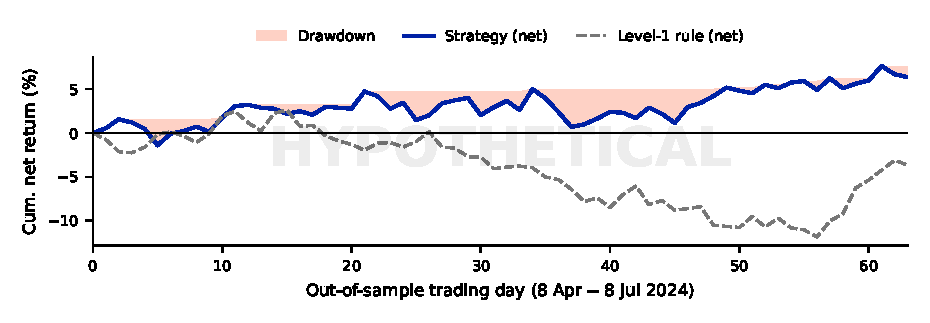
\includegraphics[width=0.82\linewidth]{equity_hypothetical.pdf}
\caption{Cumulative net returns vs.\ benchmark.}
\label{fig:equity}
\end{figure}
Figure~\ref{fig:equity} shows the hypothetical out-of-sample equity curve. The deepest drawdown is \$4{,}314 (4.3\% of reference capital); three of four calendar months are profitable (Apr +\$2{,}075, May $-$\$440, Jun +\$3{,}454, 1--8 Jul +\$1{,}278).
 
\subsection{Robustness and Attribution}
\textbf{Attribution.} SHAP summaries (Appendix~\ref{app:shap}, Figure~\ref{fig:shap}) show that signal comes mainly from imbalance and activity features: \texttt{obi\_\allowbreak l0} ranks in the top two for both directional classes, \texttt{message\_\allowbreak intensity} leads for long, and \texttt{deep\_\allowbreak ask\_\allowbreak slope} for flat. A bid-heavy top level pushes the model toward long and away from short, while \texttt{vpin} and \texttt{cancel\_\allowbreak add\_\allowbreak ratio} contribute almost nothing, so the GA can drop them, consistent with~\cite{christodoulou2025}.

\textbf{Cost and latency stress.} Table~\ref{tab:stress} reruns the out-of-sample trades under alternative round-trip costs and fixed latencies. Profit survives up to about 1.5 ticks of cost or 10\,ms of latency, but not 25\,ms.

\begin{table}[!htb]
\centering
\caption{Out-of-sample net P\&L (\$) under cost and latency stress (hypothetical)}
\label{tab:stress}
\small
\begin{tabular}{@{}lrrrr@{}}
\toprule
Round-trip cost (ticks) & 1.00 & 1.32 & 1.50 & 2.00 \\
Net P\&L & 16{,}556 & 6{,}367 & 637 & $-$15{,}282 \\
\midrule
Latency (ms), cost 1.32 & 0 & 5 & 10 & 25 \\
Net P\&L & 8{,}278 & 6{,}367 & 4{,}139 & $-$1{,}592 \\
\bottomrule
\end{tabular}
\end{table}

\textbf{Uncertainty.} The bootstrap 95\% interval for mean net P\&L per trade is $[-\$3.7,\,+\$8.7]$ and for the annualized Sharpe ratio is $[-2.4,\,5.5]$. Both include zero, so the sample is too short to separate edge from noise.
 
% ============================================================
\section{Risk Management}
% ============================================================
\subsubsection{Risk Controls}
A rule-based risk manager overrides orders without changing size:
\begin{itemize}
\item \textbf{Pre-trade gates:} Blocks trades during maintenance breaks, major macro releases (FOMC, CPI), roll weeks, wide spreads, or extreme volatility regimes.
\item \textbf{In-trade exits:} Enforces price stops, time stops ($h$), and pre-break flat triggers.
\item \textbf{Session limits:} Halts trading on daily losses exceeding 2\%, equity peak drawdowns of 5\%, or sequential loss streaks.
\end{itemize}
 
% ============================================================
\section{Liquidity and Capacity}
% ============================================================
\subsection{Liquidity Profile}
ES trades about 1.4 million contracts per day, with a one-tick spread in nearly all book events and about 25 contracts at the top of book. Our 81 contracts per day (0.006\% of ADV) fill at the first level.

\subsection{Transaction Costs and Market Impact}
Round-trip cost is 1.32 ticks (\$16.50: \$4.00 of fees plus one tick of spread), absorbing 87\% of the 1.52-tick gross edge. Table~\ref{tab:capacity} adds an uncalibrated square-root impact term of $0.008\sqrt{n}$ ticks per round trip for $n$ contracts.

\begin{table}[!htb]
\centering
\caption{Net Sharpe ratio vs.\ assumed AUM}
\label{tab:capacity}
\begin{tabular}{lrrrr}
\toprule
AUM (\$M) & 1 & 10 & 50 & 100 \\
\midrule
Net Sharpe & 1.38 & 0.95 & 0.17 & $-$0.42 \\
Max ADV participation (\%) & 0.06 & 0.58 & 2.9 & 5.8 \\
\bottomrule
\end{tabular}
\par\smallskip
\hyponote{Hypothetical. One contract per \$100k of AUM (10, 100, 500, 1{,}000 contracts); 1.4M-contract ADV.}
\end{table}
Net Sharpe falls below 1 near \$10M and turns negative by \$100M; edge is limited by cost, not liquidity.
 
% ============================================================
\section{Limitations and Next Steps}\label{sec:limits}
% ============================================================
\subsection{Limitations}
\begin{itemize}\setlength{\itemsep}{0pt}\setlength{\parskip}{0pt}
    \item \textbf{Data:} trained on one month of ES only, which captures a single market regime; MBP-10 has no queue position.
    \item \textbf{Search budget:} compute limited the GA to 100 generations, so fitness may not have converged and results may be a local optimum.
    \item \textbf{Overfitting:} many parameter sets tested on overlapping returns from a short sample, so results may not generalize.
    \item \textbf{Regime risk:} untested under stress; bursts may not revert in high-volatility markets.
    \item \textbf{Execution:} assumes 1.32-tick round trips with no impact or latency model.
\end{itemize}

\subsection{Next Steps}
\begin{itemize}\setlength{\itemsep}{0pt}\setlength{\parskip}{0pt}
    \item \textbf{More data and generations:} ideally train on 2+ years, including 2022 and Aug.\ 2024, and run the GA until fitness plateaus; test on NQ.
    \item \textbf{Validation:} hold out a clean test period and fix overlapping fitness.
    \item \textbf{Execution:} simulate passive fills with MBO data, then paper-trade live in MES.
\end{itemize}
 
\appendix
\section{SHAP Feature Attributions}\label{app:shap}
\newcommand{\shapbox}[1]{\IfFileExists{#1}{\includegraphics[width=\linewidth]{#1}}{\fbox{\parbox[c][0.69\linewidth][c]{0.96\linewidth}{\centering\small SHAP image not yet added}}}}
Figure~\ref{fig:shap} shows per-class SHAP summaries of the XGBoost model (see Section~\ref{sec:results}).
\begin{figure}[!htb]
\centering
\begin{minipage}{0.45\linewidth}\centering\shapbox{shap_short.png}\\[-2pt]{\footnotesize (a) Short class}\end{minipage}\hfill
\begin{minipage}{0.45\linewidth}\centering\shapbox{shap_long.png}\\[-2pt]{\footnotesize (b) Long class}\end{minipage}\\[4pt]
\begin{minipage}{0.45\linewidth}\centering\shapbox{shap_flat.png}\\[-2pt]{\footnotesize (c) Flat class}\end{minipage}
\caption{SHAP summary plots for the short-, long-, and flat-class XGBoost decisions.}\label{fig:shap}
\end{figure}

\addcontentsline{toc}{section}{References}
\begin{thebibliography}{99}
\small\setlength{\itemsep}{1pt}

\bibitem{chen2016xgboost}
T.~Chen and C.~Guestrin,
``XGBoost: A Scalable Tree Boosting System,''
in \textit{Proceedings of the 22nd ACM SIGKDD International Conference on Knowledge Discovery and Data Mining}, 2016, pp. 785--794.
\url{https://doi.org/10.1145/2939672.2939785}

\bibitem{christodoulou2025}
C.~N. Christodoulou-Volos,
``Optimizing Trading Strategies Using Genetic Algorithms: A Review and Implementation,''
\textit{Edelweiss Applied Science and Technology}, vol.~9, no.~10, pp.~334--345, 2025.
\url{https://doi.org/10.55214/2576-8484.v9i10.10407}

\bibitem{bailey2014dsr}
D.~H. Bailey and M.~L\'opez de Prado,
``The Deflated Sharpe Ratio: Correcting for Selection Bias, Backtest Overfitting and Non-Normality,''
\textit{Journal of Portfolio Management}, vol.~40, no.~5, pp.~94--107, 2014.
\url{https://doi.org/10.3905/jpm.2014.40.5.094}

\bibitem{Databento}
Databento. (2026). GLBX.MDP3: CME Globex market data, MBP-10 schema. Databento.
\url{https://databento.com/catalog/cme/GLBX.MDP3}

\bibitem{tillet2019triton}
P.~Tillet, H.~T. Kung, and D.~Cox,
``Triton: An Intermediate Language and Compiler for Tiled Neural Network Computations,''
in \textit{Proc.\ 3rd ACM SIGPLAN International Workshop on Machine Learning and Programming Languages (MAPL)}, 2019, pp.~10--19.
\url{https://doi.org/10.1145/3315508.3329973}

\bibitem{nautilus}
Nautech Systems, ``NautilusTrader,'' software.
\url{https://github.com/nautechsystems/nautilus_trader}

\end{thebibliography}
 
\end{document}